\documentclass[letterpaper,10pt]{article}

\usepackage[margin=0.55in]{geometry}
\usepackage{graphicx}
\usepackage{tikz}
\usepackage{xcolor}
\usepackage{helvet}
\renewcommand{\familydefault}{\sfdefault}
\pagestyle{empty}

\begin{document}

\begin{center}

\vspace*{0.5cm}

{\fontsize{24}{28}\selectfont\bfseries
RADIO OPERATOR'S\\[0.2em]
FIELD GUIDE
}

\vspace{0.4cm}

{\large
You have a radio... Now what?
}

\vspace{0.6cm}

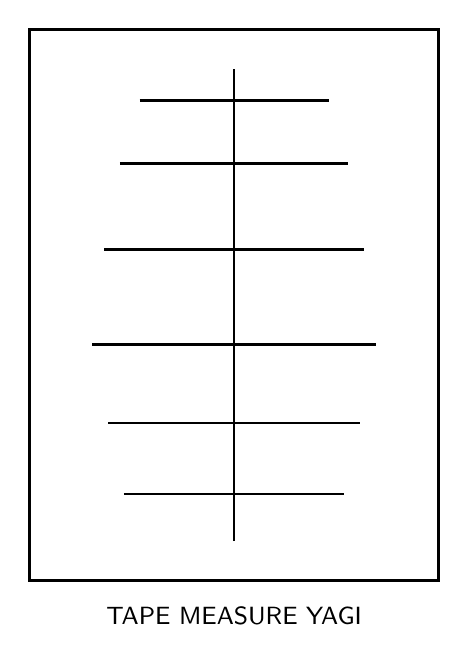
\begin{tikzpicture}
  \draw[line width=1.2pt] (0,0) rectangle (5.2,7.0);

  % simple Yagi-style sketch
  \draw[line width=1pt] (2.6,0.5) -- (2.6,6.5);
  \draw[line width=1pt] (1.2,1.1) -- (4.0,1.1);
  \draw[line width=1pt] (1.0,2.0) -- (4.2,2.0);
  \draw[line width=1pt] (0.8,3.0) -- (4.4,3.0);
  \draw[line width=1pt] (0.95,4.2) -- (4.25,4.2);
  \draw[line width=1pt] (1.15,5.3) -- (4.05,5.3);
  \draw[line width=1pt] (1.4,6.1) -- (3.8,6.1);

  \node[align=center,font=\small] at (2.6,-0.45) {TAPE MEASURE YAGI};
\end{tikzpicture}

\vspace{0.7cm}

\begin{minipage}{0.85\textwidth}
\centering
\small
Make a contact. Build an antenna. Find a fox.\\
Skip the textbook. Start doing.
\end{minipage}

\vfill

\hrule
\vspace{0.25cm}

{\small
Ham Radio Village / DEF CON Edition \hfill Version 0.1
}

\vspace{0.15cm}

{\footnotesize
Open-source printable zine for new technicians
}

\end{center}

\end{document}
